\documentclass[a4paper,10pt]{report}
\usepackage[utf8]{inputenc}
\usepackage[italian]{babel}
\usepackage{graphicx}
\usepackage[hidelinks]{hyperref}
\usepackage{listings}
\usepackage{color}
\usepackage{graphicx}

\definecolor{dkgreen}{rgb}{0,0.6,0}
\definecolor{gray}{rgb}{0.5,0.5,0.5}
\definecolor{mauve}{rgb}{0.58,0,0.82}

\lstset{frame=tb,
  language=Java,
  aboveskip=3mm,
  belowskip=3mm,
  showstringspaces=false,
  columns=flexible,
  basicstyle={\small\ttfamily},
  numbers=none,
  numberstyle=\tiny\color{gray},
  keywordstyle=\color{blue},
  commentstyle=\color{dkgreen},
  stringstyle=\color{mauve},
  breaklines=true,
  breakatwhitespace=true
  tabsize=3,
  moredelim=[is][\textcolor{gray}]{&&}{&&}
}

% Title Page
\title{Analisi e sviluppo di una web application \\
basata sui framework JPA, JSF, CDI, \\
per l'amministrazione di attività di trasferimento tecnologico}
\author{Tommaso Levato, Alessio Sarullo, Giulio Galvan}


\begin{document}
\maketitle

\begin{abstract}
\end{abstract}

\tableofcontents

\chapter{Introduzione}
\chapter{Analisi}
\section{Casi d'uso}
Di seguito si elencano i casi d'uso per ciascun tipo di utente che interagisce col sistema. 
\begin{enumerate}

\item \textbf{Utente generico}\\
Si racchiudono nella figura dell'Utente generico i casi d'uso che sono comuni a tutti gli altri tipi di utenti. Tali casi d'uso sono riportati in figura \ref{use_case_diag_generic}

\begin{figure}[h]
  \caption{Diagramma dei casi d'uso dell'Utente generico}
  \label{use_case_diag_generic}
  \centering
    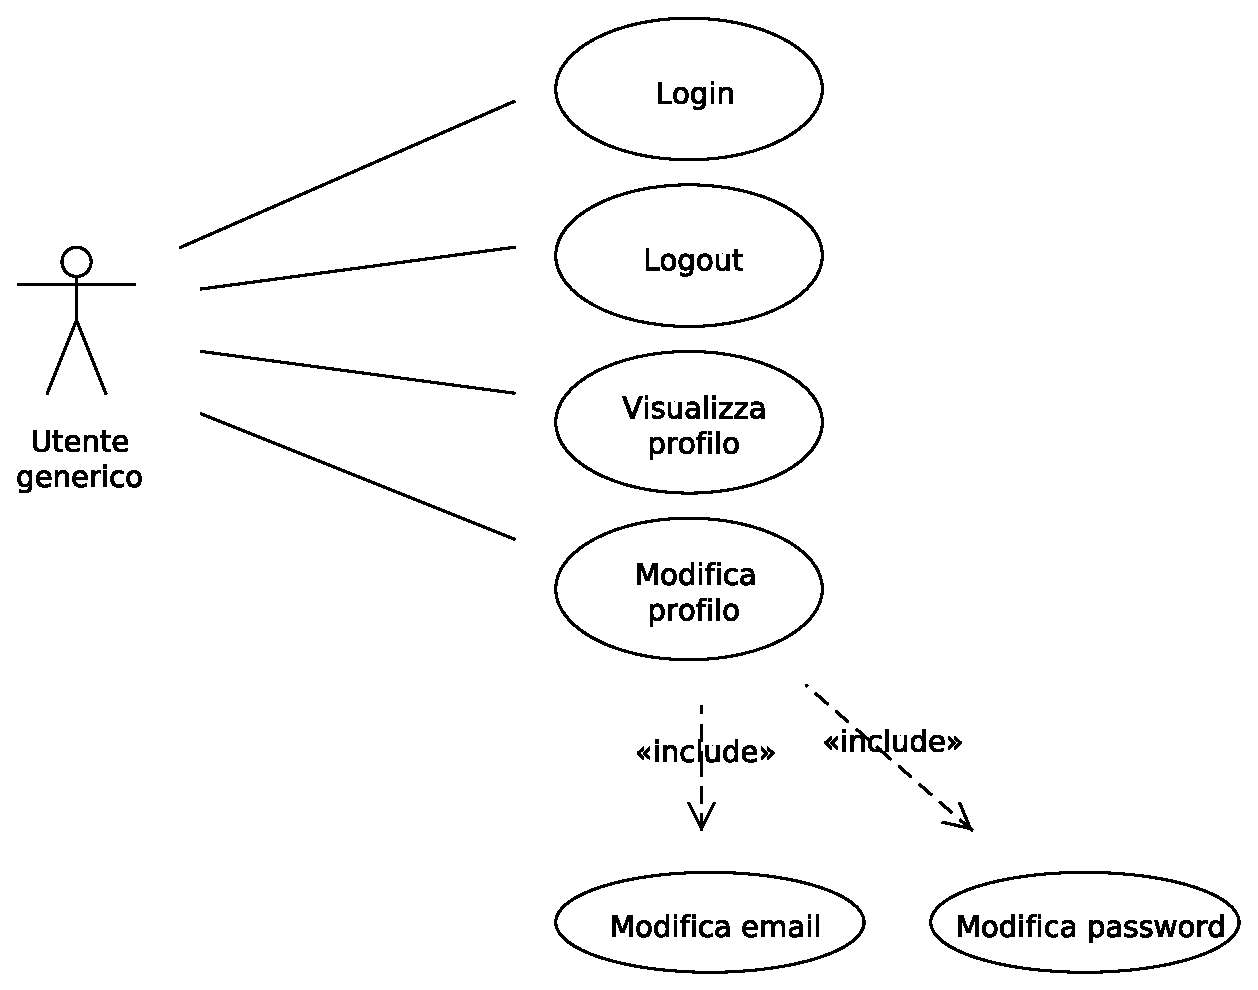
\includegraphics[width=0.7\textwidth]{images/casi_uso_utente_generico.eps}
\end{figure}

\begin{enumerate}

 \item Login\\ \label{UC_login}
    Percorso base:
    l'Utente Generico, dopo aver raggiunto l'indirizzo web dell'applicativo, inserisce il proprio numero di matricola e password, quindi clicca sul pulsante ``Login". Viene visualizzata la pagina iniziale.\\
    Percorso alternativo:
    l' Utente Generico inserisce i propri dati personali ma commette un errore, quindi clicca su ``Login". Viene visualizzato un messaggio nel quale si avvisa l'utente dell'errore commesso.
    
 \item Visualizzazione del profilo\\ \label{UC_view_profile}
    Dopo aver effettuato il login , l'Utente Generico clicca sul pulsante ``Profilo" nella toolbar in alto; si presenta una schermata contente i dati personali dell'Utente.
 \item Modifica dell'indirizzo e-mail\\ \label{UC_edit_email}
  Percorso base:
  dopo aver effettuato il login , l'Utente Generico clicca sul pulsante ``Profilo" nella toolbar in alto; si presenta una schermata contente i dati personali dell'Utente.
  L'Utente cambia il proprio indirizzo e-mail. Una volta effettuate le modifiche desiderate l'Utente clicca su ``Salva". Le modifiche vengono salvate e viene visualizzata la schermata precedente.\\
  
  Percorso alternativo:
  l'Utente inserisce una e-mail non valida. L'Utente è avvertito dell'errore con un messaggio ed è invitato a riprovare.
\end{enumerate}



\item \textbf{Operatore}\\
Una rappresentazione grafica dei casi d'uso dell'Operatore è disponibile in figura \ref{use_case_diag_operator}
\begin{figure}[h]
  \caption{Diagramma dei casi d'uso dell'Operatore}
  \label{use_case_diag_operator}
  \centering
    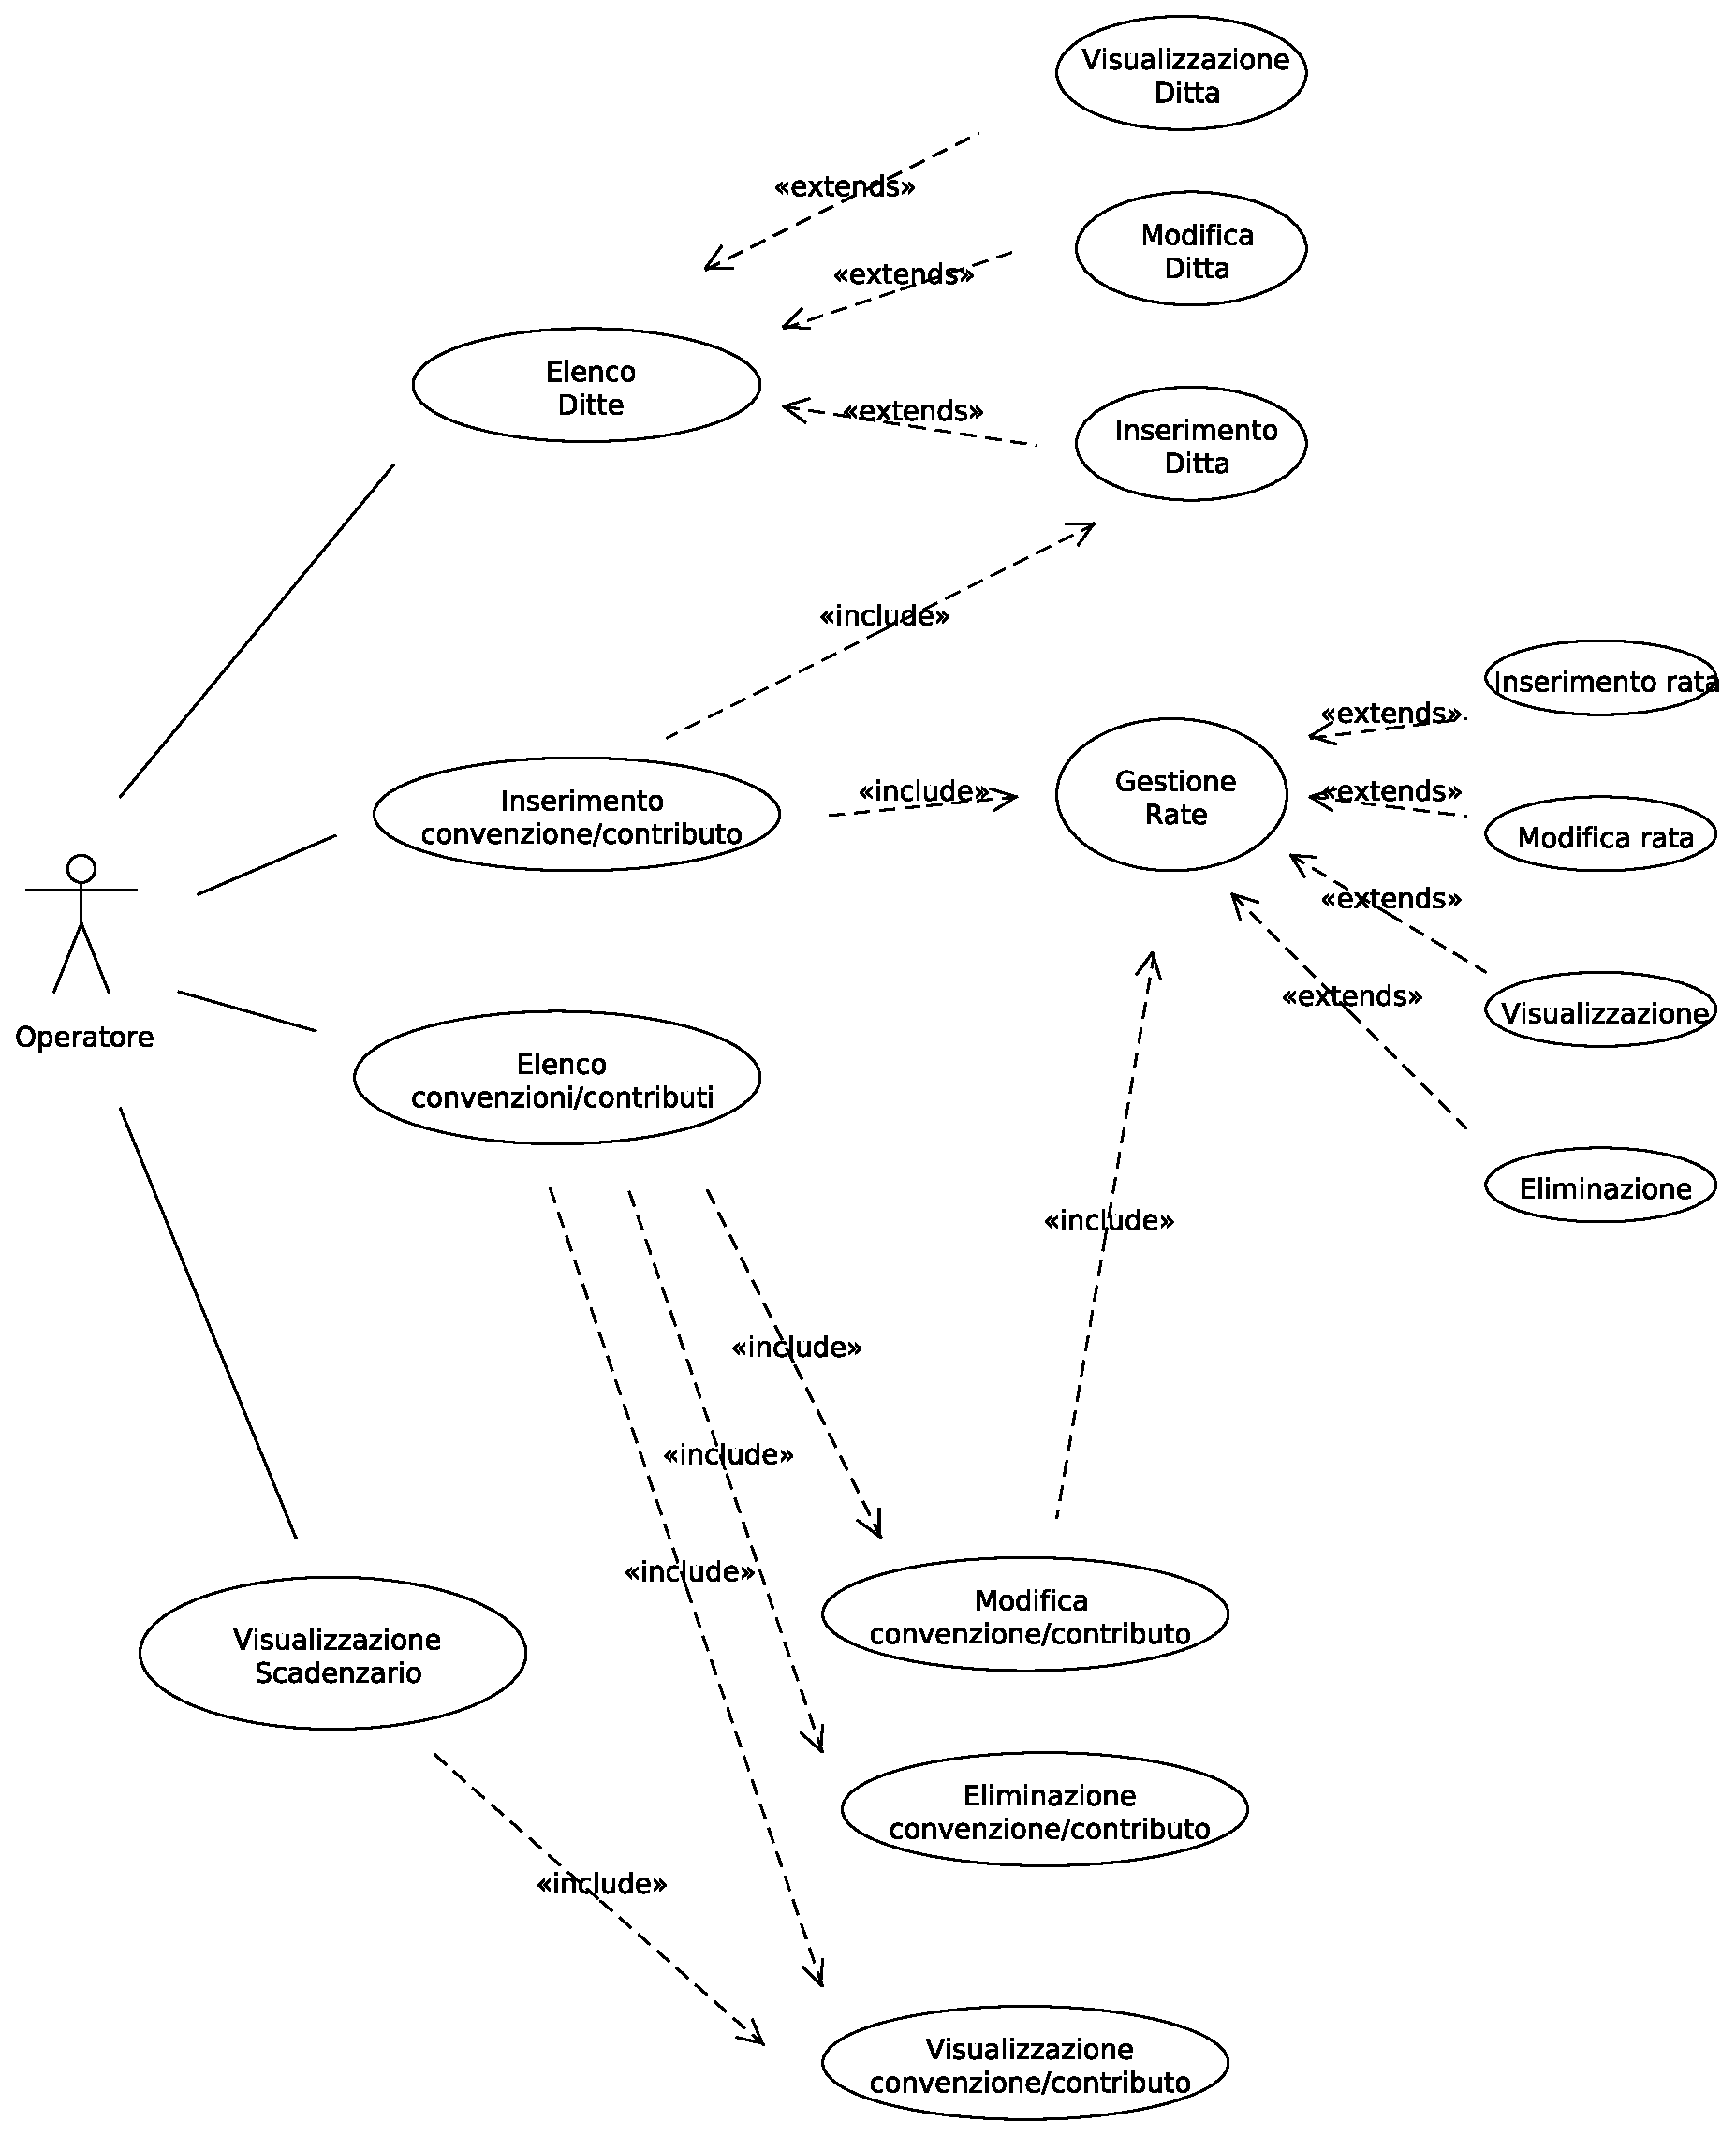
\includegraphics[width=1\textwidth]{images/casi_uso_operatore.eps}
\end{figure}

\begin{enumerate}
  \item Inserimento di una nuova Convenzione/Contributo\\ \label{UC_new_contract}
  
  Percorso base:
  l'Operatore, una volta effettuato il login, clicca su ``Crea una convenzione/contributo"; viene visualizzata una schermata suddivisa in varie schede,
  ognuna corrispondente ad un passo della procedura. E' possibile passare da una vista all'altra mediante i pulsanti ``Avanti" e ``Indietro". I passi sono:
  \begin{enumerate}
    \item Inserimento dei dati della convenzione/contributo\\
      
      In questa scheda sono elencati tutti i campi necessari per la definizione di una convenzione/contributo, 
      che l'Operatore deve compilare. Tali campi sono:
      \begin{itemize}
	\item Il titolo
	\item Il titolo riassuntivo
	\item Il numero di protocollo
	\item L'UAR
	\item La tipologia
	\item Il responsabile scientifico\\
	  Per selezionare un responsabile scientifico è possibile usare l'apposito menù a tendina o, in alternativa, qualora la persona cercata non sia nell'elenco, aggiungerla cliccando sul pulsante ``Aggiungi".
	\item Il referente
	\item La ditta\\
	  Per selezionare una ditta si può usare l'apposito menù a tendina o, se la ditta cercata non fosse presente nell'elenco, aggiungerne una nuova cliccando sul pulsante ``Aggiungi".Per ulteriori dettagli si rimanda \ref{UC_new_company}.
	\item Il nome del progetto CIA
	\item Il Repertorio
	\item Il totale imponibile
	\item L'Iva
	\item La data di approvazione
	\item La data di inizio
	\item La data di scadenza
      \end{itemize}
      
      Nota : i campi riguardanti l'Iva non sono presenti nel caso del contributo.
      
    \item Inserimento della tabella di ripartizione\\
     
      Questa scheda contiene le voci della tabella di ripartizione. L'Operatore può modificare alcuni valori percentuali 
      in base ai quali dividere l'importo totale. Le voci non modificabili sono calcolate in relazione ai campi modificabili facendo riferimento alle norme di ateneo. Le voci modificabili sono:
      \begin{itemize}
	\item Personale: stabilisce la quota destinata al personale; è l'unico campo principale che l'operatore può modificare e in base al quale vengono calcolati gli altri.
	\item Missioni, Materiale di consumo, etc. sono sotto-campi di Beni e Servizi e servono per meglio specificare come verrà ripartita la quota destinata a ``Beni e Servizi".
      \end{itemize}
      
      Nota : questa scheda è assente nel caso del contributo, non essendo prevista una ripartizione.
    \item Gestione delle rate\\
      
      Questo passo della procedura è facoltativo: viene data la possibilità all'operatore di inserire delle rate per la convenzione/contributo
      che sta creando. Una volta inserite una o più rate
      queste vengono visualizzate in una tabella e l'Operatore
      ha la possibilità di modificare, visualizzare o eliminare una rata cliccando sui tasti ``Modifica",``Visualizza" ed ``Elimina" che compaiono sulla sinistra, nella riga della tabella
       corrispondente alla rata in questione. Per i dettagli riguardo alle operazioni sulle rate si rimanda ai corrispettivi casi d'uso.

      
    \item Inserimento della documentazione relativa alla convenzione\\
	  
	  Questa scheda elenca i documenti allegati alla convenzione. L'Operatore può aggiungere o eliminare un documento 
	  cliccando sugli appositi tasti. Premendo il tasto ``Salva" la convenzione viene salvata e la procedura termina. Si ritorna alla schermata precedente.
  \end{enumerate}
		 
  Percorso alternativo 1:
  Durante uno qualsiasi dei passi, l'Operatore  clicca sul tasto ``Annulla", che comporta, a seguito di una conferma, il ritorno alla schermata precedente
  senza che la convenzione/contributo venga inserita o i cambiamenti effettuati salvati.
  
  Percorso alternativo 2:
  l'Operatore clicca sul tasto ``Salva" senza aver compilato alcuni dei campi obbligatori, o avendo inserito dei valori non consentiti; viene visualizzato un messaggio di errore 
  e il documento non viene salvato. La schermata non viene cambiata, dando la possibilità all'Operatore di procedere alla correzione.
     
  \item Visualizzazione delle convenzioni/contributi\\ \label{UC_view_contract_list}

  Percorso base:
  l'Operatore clicca su ``Visualizza contratti"; viene mostrata una lista delle convenzioni/contributi correntemente stipulate in 
  riferimento al dipartimento di afferenza dell'Operatore, con opportuni filtri 
  per agevolare la ricerca (tra cui un filtro per data di scadenza) e ordinabili per data.
  L'Operatore può selezionare una convenzione e, mediante gli appositi pulsanti che appaiono sulla sinistra, modificare, visualizzare o eliminare una convenzione. Per i dettagli si rimanda casi d'uso relativi a tali operazioni.\\	

  Percorso alternativo:
  L'Operatore clicca sul tasto ``Home", si torna alla pagina iniziale.
 
  \item Modifica di una convenzione/contributo\\ \label{UC_edit_contract}
  
  Percorso base:
  l'Operatore a partire dalla schermata ``Visualizzazione Contratti" clicca sul pulsante ``Modifica" che appare sulla sinistra nella riga 
  della tabella corrispondente alla convenzione/contributo desiderata. Viene visualizzata una schermata suddivisa in schede analoga a quella
  descritta nel caso della ``Creazione di una convenzione/contributo", con la differenza che in questo caso è possibile spostarsi da una scheda all'altra
  cliccando sulla scheda stessa. Inoltre è presente la scheda aggiuntiva ``Riepilogo" che contiene alcune informazioni di riepilogo come il residuo
  totale della convenzione/contributo o il totale fatturato.
  L'Operatore effettua i cambiamenti desiderati quindi clicca sul pulsante ``Salva"; i dati vengono salvati e si ritorna all'elenco delle convenzioni/contributi\\

  Percorso alternativo 1:
  l'Operatore clicca sul tasto \textquotedblleft Annulla" da qualsiasi scheda;  si torna alla schermata \textquotedblleft Visualizzazione Contratti" senza salvare le modifiche effettuate.\\
  
  Percorso alternativo 2:
  l'Operatore clicca su \textquotedblleft Salva" ma alcuni valori immessi non sono corretti, viene visualizzato un messaggio di errore e non si torna alla schermata \textquotedblleft Visualizzazione delle
  convenzioni/contributi" dando la possibilità all'Operatore di correggere gli errori commessi prima di salvare nuovamente.
  
  \item Visualizzazione di una convenzione/contributo\\ \label{UC_view_contract}
 
  Del tutto analogo a ``Modifica di una convenzione/contributo" con la differenza che in questo caso non è possibile modificare i dati della
  convenzione/contributo.
  
  \item Eliminazione di una convenzione/contributo\\ \label{UC_delete_contract}
  
  Percorso base:
  l'Operatore a partire dalla schermata ``Visualizzazione Contratti" clicca sul pulsante ``Elimina" che appare sulla sinistra nella riga 
  della tabella corrispondente alla convenzione/contributo desiderata. Appare una finestra di dialogo che chiede di confermare l'operazione. L'Operatore clicca sul pulsante ``Sì", la convenzione/contributo viene eliminato e si
  ritorna alla schermata precedente.
  
  Percorso alternativo:
  l'Operatore, dopo aver cliccato su ``Elimina", essendosi accorto di aver commesso un errore, clicca sul pulsante ``No". La convenzione/contributo non viene eliminata e si ritorna alla schermata precedente.
  
  
  
\item Inserimento di una rata\\ \label{UC_new_installment}
Percorso base:
l'Operatore può inserire una rata sia in fase di creazione della convenzione/contributo sia in fase di modifica; in entrambi i casi dopo aver raggiunto
la scheda ``Rate" l'Operatore clicca sul pulsante ``Aggiungi una rata".  
Viene visualizzata una finestra di dialogo suddivisa in varie schede,
ognuna corrispondente ad un passo della procedura. E' possibile passare da una scheda all'altra mediante i pulsanti \textquotedblleft Avanti" e \textquotedblleft Indietro". I passi sono:
\begin{enumerate}
  \item Inserimento dei dati della rata\\
  
  L'operatore inserisce i seguenti campi
    \begin{itemize}
    \item Importo
    \item Iva
    \item Data
    \item Numero Reversale
    \item Data Reversale
    \item Numero di Sospeso
    \item Numero di fatturato
    \item Data fatturata
    \item È stata pagata la fattura?
    \item Deve essere allegata la fattura?
    \item Note
    \end{itemize}
    
   Nota : i campi riguardanti l'Iva non sono presenti nel caso del contributo.

   
  \item Inserimento della tabella di ripartizione\\
  
  Il procedimento è del tutto analogo a quello descritto nel caso d'uso \textquotedblleft Inserimento della tabella di ripartizione" per l'inserimento di 
  una nuova convenzione/contributo. 
\end{enumerate}

L'Operatore clicca pulsante \textquotedblleft Salva".Le modifiche vengono salvate e si torna alla schermata precedente;

Percorso alternativo:
l'Operatore clicca sul pulsante ``Annulla", viene chiusa la finestra di dialogo senza che la rata sia stata inserita.

\item Modifica di una rata\\ \label{UC_edit_installment}

Percorso base:
l'Operatore accede alla schermata ``Visualizzazione contratti" cliccando sul pulsante apposito nella pagina iniziale, quindi seleziona la convenzione/contributo alla quale la rata appartiene e clicca sul pulsante ``Modifica" che compare
all'interno della riga selezionata. Viene così visualizzata la schermata ``Modifica di una convenzione/contributo"; l'Operatore raggiunge la scheda ``rate" e clicca sul pulsante ``Modifica" che compare selezionando la riga della tabella
corrispondente alla rata desiderata. Viene visualizzata una finestra di dialogo composta di varie schede analoghe a quelle descritte nel caso dell'inserimento. E' possibile passare da una scheda all'altra cliccando su di esse.
Dopo avere effettuato le modifiche richieste l'Operatore clicca sul pulsante ``Salva", la convenzione/contributo viene aggiornata e viene visualizzata la schermata precedente.

Percorso alternativo:
l'Operatore clicca sul pulsante ``Annulla", le modifiche vengono scartate e si torna alla schermata precedente.

\item Visualizzazione di una rata \label{UC_view_installment}

Una volta raggiunta la scheda ``rate" relativa alla convenzione/contributo di interesse l'Operatore, dopo aver selezionato la rata desiderata, clicca sul pulsante ``Visualizza". Viene presentata una finestra di dialogo analoga a quella descritta nel caso della modifica 
con la differenza che i campi non sono modificabili. E' possibile tornare alla schermata precedente cliccando sul pulsante ``Indietro".

\item Eliminazione di una rata\\ \label{UC_delete_installment}

Raggiunta la scheda ``rate" relativa alla convenzione/contributo di interesse, l'Operatore, dopo aver selezionato la rata di interesse, clicca sul pulsante ``Elimina'; appare una finestra di dialogo che chiede di confermare
l'eliminazione, l'Operatore clicca "Sì"la rata viene eliminata e si torna alla schermata precedente.

\item Inserimento di una Ditta\\ \label{UC_new_company}
Percorso base:
l'Operatore clicca su ``Visualizza elenco Ditte" dalla pagina iniziale; viene visualizzata una schermata contenente un elenco delle ditte inserite. L'Operatore clicca sul pulsante ``Aggiungi" in basso a sinistra. Viene visualizzata
una finestra di dialogo contente i seguenti campi obbligatori:
\begin{itemize}
 \item Denominazione
 \item Ragione sociale
 \item Sede Legale
 \item Codice fiscale
 \item Partita IVA
\end{itemize}
l'Operatore dopo aver riempito i campi clicca su ``Salva", la nuova ditta viene salvata e si ritorna alla schermata precedente.

Percorso alternativo:
l'Operatore clicca su ``Salva" senza aver riempito tutti i campi obbligatori, viene visualizzato un messaggio di errore che invita l'utente inserire tali campi.

Percorso alternativo 2:
l'Operatore clicca su ``Salva" avendo inserito un codice fiscale di una ditta già inserita. Viene visualizzato un opportuno messaggio di errore.

Percorso alternativo 3:
si può inserire una ditta anche in fase di creazione di una convenzione/contributo cliccando sul pulsante ``Aggiungi" accanto al campo ``ditta" nella scheda ``Dati generali".

\item Modifica di una Ditta\\ \label{UC_edit_company}

Percorso base:
l'Operatore clicca su ``Visualizza elenco Ditte" dalla pagina iniziale; viene visualizzata una schermata contenente un elenco delle ditte inserite. L'Operatore dopo aver posizionato il cursore sulla riga dell'elenco
corrispondente alla ditta di interesse clicca sul pulsante ``Modifica"che appare a sinistra sulla riga selezionata. Viene visualizzata
una finestra di dialogo analoga a quella dell'inserimento.

l'Operatore dopo aver modificato i campi desiderati clicca su ``Salva", la  ditta viene salvata e si ritorna alla schermata precedente.

Percorso alternativo:
l'Operatore clicca su ``Salva" senza aver riempito tutti i campi obbligatori, viene visualizzato un messaggio di errore che invita l'utente a inserire tali campi.

Percorso alternativo 2:
l'Operatore clicca su ``Salva" avendo inserito un codice fiscale di una ditta già inserita. Viene visualizzato un opportuno messaggio di errore.

\item Visualizzazione di una Ditta\\ \label{UC_view_company}
  Percorso base:
  l'Operatore raggiunge l'elenco delle ditte quindi clicca sul pulsante ``Visualizza ditta" che compare sulla sinistra selezionando la riga dell'elenco corrispondente alla ditta desiderata.

\item Visualizzazione dell'elenco delle ditte\\ \label{UC_view_company_list}
  Percorso base:
  l'Operatore dalla pagina iniziale clicca sul pulsante ``Visualizza elenco ditte". Viene presentata una schermata contente un elenco di ditte filtrabili per nome attraverso l'apposito filtro di ricerca.
  
\item Visualizzazione dello Scadenzario\\ \label{UC_view_deadlines}
  Percorso base:
  l'Operatore dalla pagina iniziale clicca sul pulsante ``Visualizza scadenzario", Viene presentata una schermata contente un elenco di contratti che hanno delle rate con scadenze attive. E' possibile filtrare i risultati in base a vari
  criteri di ricerca. Selezionando una convenzione/contributo e cliccando sul pulsante ``Visualizza" che compare sulla destra è possibile visualizzare una convenzione/contributo, per i dettagli su questa operazione si rimanda a \ref{UC_view_contract}

\end{enumerate}

 
\item \textbf{Docente}\\
I casi d'uso del Docente sono rappresentati in figura \ref{use_case_diag_teacher}
\begin{figure}[h]
  \caption{Diagramma dei casi d'uso del Docente}
  \label{use_case_diag_teacher}
  \centering
    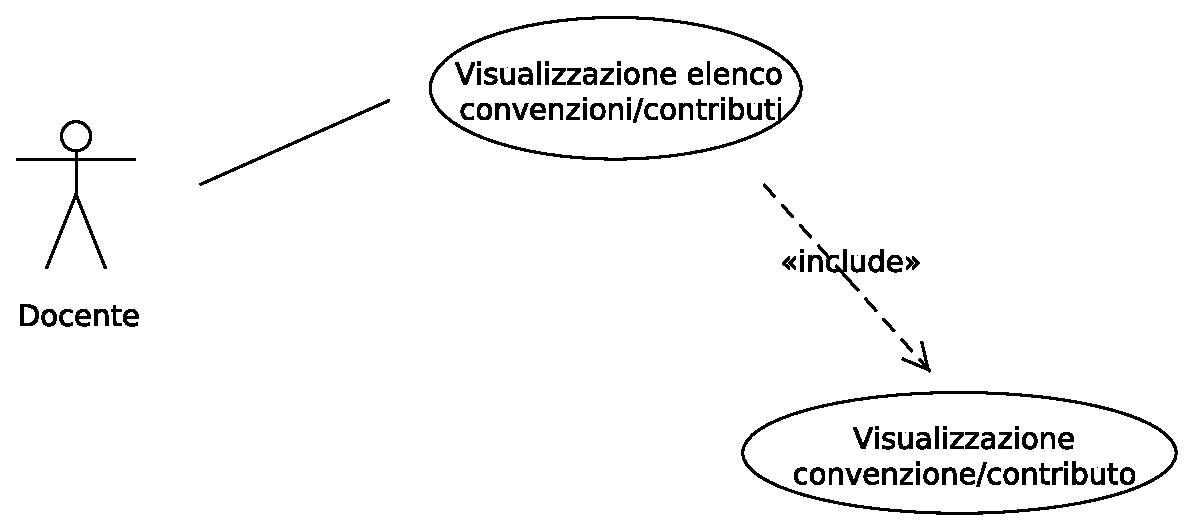
\includegraphics[width=0.8\textwidth]{images/casi_uso_docente.eps}
\end{figure}

\begin{enumerate}
 
 \item Visualizzazione dell'elenco delle convenzioni/contributi di cui il docente è responsabile scientifico\\ \label{UC_view_own_contract_list}
 
 Il docente, dopo aver effettuato il login, può cliccare sul pulsante ``Visualizzazione della lista delle convenzioni/contributi"; la schermata
 che viene visualizzata contiene una tabella che elenca le convenzioni/contributi del docente. E' possibile filtrare le convenzioni/contributi
 secondo vari criteri(data, tipo, scadenze più vicine, ...).Inoltre è possibile visualizzare i dettagli di una convenzione/contributo cliccando sul
 pulsante ``Visualizza" che appare posizionando il puntatore su una riga della tabella.
 
 \item Visualizzazione di una convenzione/contributo di cui il docente è responsabile scientifico\\ \label{UC_view_own_contract}
 
 Il docente dalla schermata ``Visualizzazione delle convenzioni/contributi" può cliccare sul pulsante ``Visualizza" relativo ad una convenzione/contributo; compare una schermata suddivisa in schede analoga a quella della modifica/creazione
 della convenzione. Il docente può navigare fra le schede cliccandoci sopra. Non è permessa nessuna modifica ai dati della convenzione/contributo, tuttavia il docente può gestire gli allegati dalla scheda ``Allegati", per i dettagli
 si rimanda a \ref{UC_manage_attachments}. Cliccando su ``Salva"
 gli allegati inseriti dal docente vengono memorizzati, al contrario cliccando su ``Indietro" le modifiche vegono scartate.
 
 \item Gestione allegati\\ \label{UC_manage_attachments}
  
 Percorso base:
 il Docente raggiunge la scheda ``Allegati" di una convenzione/contributo quindi:
  \begin{itemize}
   \item clicca su ``Aggiungi", viene presentata una finestra di dialogo che consente di selezionare un file da inserire come allegato.
   \item clicca sul pulsante ``Download" che compare sulla destra selezionando una riga della tabella degli allegati. Il file corrispondente a tale riga viene scaricato sul computer dell'utente.
   \item clicca sul pulsante ``Rimuovi" che compare sulla destra selezionando una riga della tabella degli allegati. Il file corrispondente viene rimosso dagli allegati della convenzione/contributo
  \end{itemize}
 il docente clicca quindi su ``Salva", le modifiche vengono apportate e si ritorna alla schermata precedente.
 
 Percorso alternativo:
 il Docente, dopo aver effettuato alcune modifiche clicca su ``Indietro", le modifiche non vengono salvate e si ritorna alla schermata precedente.

 
\end{enumerate}



\item \textbf{Amministratore}\\
Una rappresentazione dei casi d'uso dell'Amministratore è disponibile in figura \ref{use_case_diag_admin}
\begin{figure}[h]
  \caption{Diagramma dei casi d'uso dell'Amministratore}
  \label{use_case_diag_admin}
  \centering
    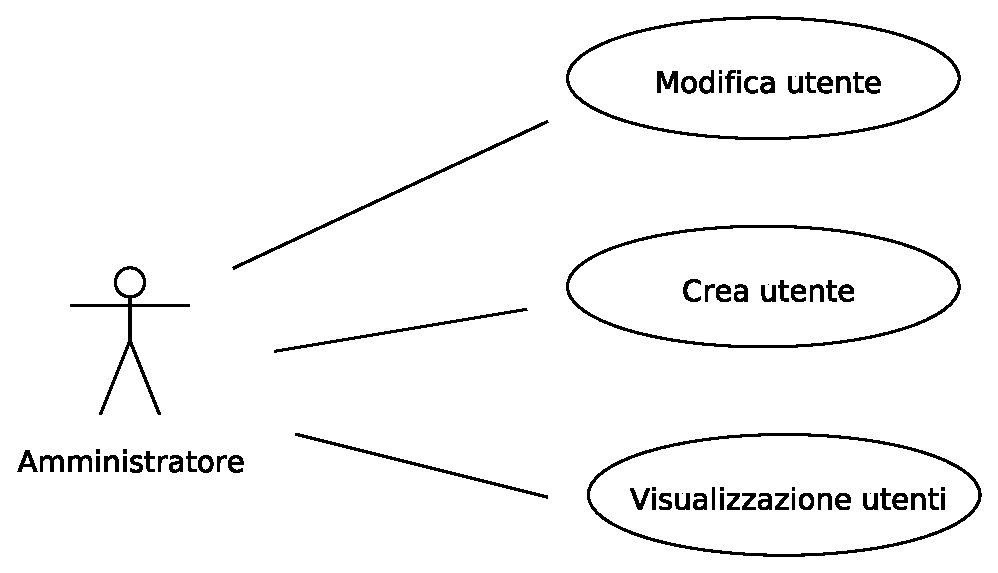
\includegraphics[width=0.6\textwidth]{casi_uso_amministratore.eps}
\end{figure}


\begin{enumerate}
 \item Inserimento di un nuovo utente\\ \label{UC_new_user}
 
 
 Percorso base:
 l'Amministratore, dopo aver effettuato il login, clicca sul pulsante ``Crea nuovo utente"; viene visualizzata una schermata che permette
 di inserire i dati dell'utente:
 \begin{itemize}
  \item Nome
  \item Cognome
  \item Matricola
  \item E-mail
  \item	Password\\
    In realtà i campi che l'Amministratore deve riempire sono due: un campo password ed un campo di verifica che deve corrispondere col precedente.
  \item Ruolo\\
    L'Amministratore può scegliere il ruolo dal rispettivo menù a tendina, i ruoli disponibili sono Operatore, Amministratore, Docente.
 \end{itemize}
 
 Una volta completato l'inserimento, l'Amministratore clicca sul pulsante ``Salva", il nuovo utente viene registrato nel sistema. 

 Percorso alternativo 1:
 l'Amministratore inserisce solo il campo matricola e quindi clicca il pulsante ``Importa Utente da LDAP". I rimanenti campi, se la matricola è valida,
 vengono automaticamente importati dal servizio LDAP offerto da SIAF. L'Amministratore conclude la procedura cliccando sul pulsante ``Salva"
 
 Percorso alternativo 2:
 l'Amministratore in qualunque momento della procedura clicca sul pulsante ``Annulla"; viene presentata a video la schermata precedente,
 nessun utente viene aggiunto al sistema.
 
 \item Visualizzazione della lista degli utenti \label{UC_view_user_list}
  L'Amministratore, una volta effettuato il login, clicca sul pulsante ``Visualizza utenti"; viene presentata una schermata contenente una lista  degli
  utenti inseriti nel sistema. L'Amministratore clicca sul pulsante ``Indietro" per tornare alla pagina iniziale.
\end{enumerate}

\item \textbf{Tempo}\\
I casi d'uso del Tempo sono rappresentati in figura \ref{use_case_diag_teacher}
\begin{figure}[h]
  \caption{Diagramma dei casi d'uso del Tempo}
  \label{use_case_diag_time}
  \centering
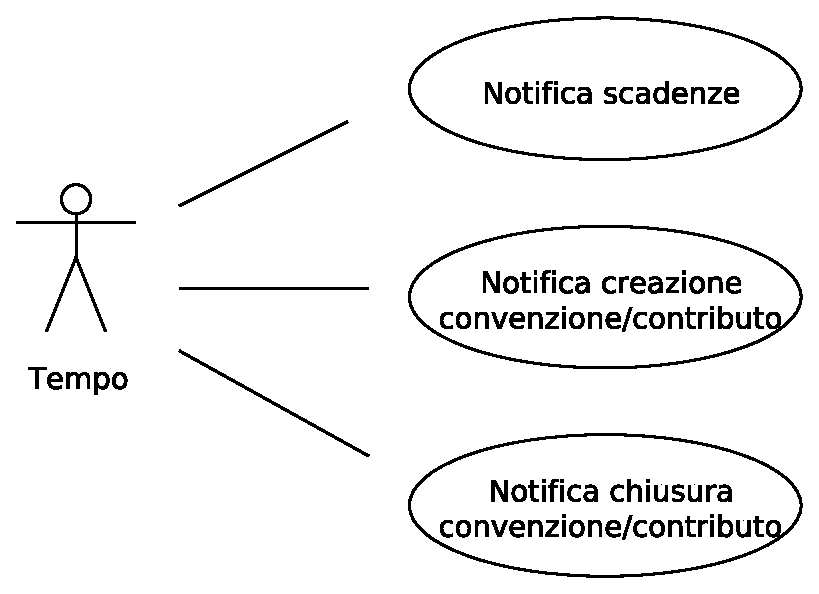
\includegraphics[width = 0.5\textwidth]{images/casi_uso_tempo.eps}
\end{figure}
\begin{enumerate}
 \item Notifica delle scadenze\\ \label{UC_notify_deadlines}
 
    Ad intervalli periodici stabiliti, i docenti che hanno convenzioni/contributi attive con rate in scadenza ravvicinata, vengono avvertiti tramite posta elettronica.
  
 
 \item Notifica della creazione di una nuova convenzione/contributo\\ \label{UC_notify_new_contract}
 
    Al momento del completamento della creazione di una nuova convenzione/contributo viene inviata una e-mail all'indirizzo di posta elettronico del responsabile scientifico indicato per la convenzione/contributo. Tale e-mail contiene
    le informazioni principali che caratterizzano la convenzione/contributo.
  
  
 \item Notifica della chiusura di una convenzione/contributo\\ \label{UC_notify_closed_contract}
 
    Al momento della chiusura di una convenzione/contributo (ovvero quando il fatturato è pari all'importo totale) viene inviata una e-mail all'indirizzo di posta elettronico del responsabile scientifico che notifica la chiusura della
    convenzione/contributo riportando alcuni dati di questa.
\end{enumerate}


\end{enumerate}


\chapter{Tecnologie}
\section{JPA}
\section{CDI}
\subsection{Introduzione}

La specifica \textsl{Contexts and Dependecy Injection} (o, più semplicemente, \textsl{CDI}) è stata introdotta nella versione 6 di Java EE per unificare il livello applicazione (che fa uso degli \textsl{Enterprise Java Bean}, o \textsl{EJB}) e il livello web (con particolare riferimento alla tecnologia JSF, che fa uso dei \textsl{Managed bean}).\\
Esistono attualmente varie versioni di CDI. Nello sviluppo dell'applicazione è stata usata \textsl{JBoss Weld}, che è quella di riferimento ed è inoltre inclusa di default in \textsl{JBoss AS}.\\
In seguito, verranno descritti in modo sufficientemente approfondito le caratteristiche principali di CDI. Per una trattazione più dettagliata e completa, si rimanda alla specifica \cite{cdi} e alla documentazione dell'implementazione di riferimento \cite{weld}.

\subsection{Caratteristiche}

I principali servizi offerti da CDI sono due:

\begin{itemize}
\item \textbf{Contesto}: CDI è in grado di conferire agli oggetti Java un ciclo di vita legato ad un particolare contesto.
\item \textbf{Iniezione di dipendenza}: tramite CDI è possibile delegare al framework il compito di istanziare gli oggetti, creando così un meccanismo di iniezione di dipendenza. Tale operazione può essere eseguita sia durante lo sviluppo che durante la fase di \textit{deploy} dell'applicazione. Questi oggetti gestiti dal framework invece che direttamente dal programmatore vengono denominati \textsl{bean}.
\end{itemize}

Inoltre CDI:

\begin{itemize}
\item consente l'integrazione con l'\textsl{Expression Language} (o \textsl{EL}), permettendo di far riferimento agli oggetti dalle pagine JSF in modo diretto.
\item favorisce il disaccoppiamento sia al livello client-server, permettendo varie implementazioni lato server attraverso l'utilizzo dei \textit{qualifier}, sia per quanto riguarda il ciclo di vita dei bean, attraverso una sua gestione mediante l'utilizzo di vari contesti.
\item permette un forte controllo sui tipi, eliminando la necessità di identificatori di tipo stringa per il collegamento tra i vari bean tramite l'utilizzo delle annotazioni Java.
\end{itemize}

\subsection{Bean}

\subsubsection{Definizione}
Alla base di CDI vi sono oggetti particolari chiamati \textsl{bean}.\\
Un bean, nella sua accezione più ampia, è un \textquotedblleft componente software riusabile che può essere gestito dal container\textquotedblright{} (adattamento libero della definizione fornita dalla specifica \textsl{JavaBeans}, consultabile all'indirizzo \cite{javaBeans}).\\
I bean di CDI rispettano questa specifica, ma hanno un'importante proprietà aggiuntiva: lo \textit{scope}, che li lega ad uno specifico contesto, il quale ne determina il ciclo di vita e la visibilità ai client.
CDI mette a disposizione quattro \textit{scope}:
\begin{itemize}
\item \textit{Request scope} Il tempo di vita del bean equivale ad una singola richiesta HTTP
\item \textit{Conversation scope} Una \textsl{conversazione} di CDI può essere di due tipi: \textit{transient} e \textit{long-running}. Normalmente, una conversazione è \textit{transient} e ha la stessa durata di una richiesta HTTP. Tuttavia, una conversazione \textit{transient} può divenire \textit{long-running} tramite una chiamata al metodo \lstinline{begin()}, e rimane tale finché non viene chiamato il metodo \lstinline{end()}, riportandola allo stato \textit{transient}.
\item \textit{Session scope} È legato alla sessione HTTP. Un bean \textit{session scoped} rimane quindi attivo attraverso più richieste HTTP ed è visibile tra più viste che condividono la stessa sessione.
\item \textit{Application scope} Un bean \textit{application scoped} viene creato una volta sola per tutta la durata dell'applicazione.
\end{itemize}

Oltre agli \textit{scope} \textquoteleft classici\textquoteright{} appena elencati, ve ne sono altri chiamati \textit{pseudo-scope}. Tra questi, il più importante è lo \textit{pseudo-scope} \textit{dependent}: un bean \textit{dependent} viene istanziato per servire un solo client o bean, ed il suo ciclo di vita è quindi legato a quello del client/bean. Se ad un bean non viene assegnato esplicitamente uno \textit{scope}, viene considerato \textit{dependent}.\\\\

Un bean CDI non è solo definito dal suo \textit{scope}: di seguito sono elencati gli altri principali attributi di un bean CDI.
\begin{itemize}
\item \underline{Un insieme (non vuoto) di \textit{bean type}}. Un \textit{bean type} è un tipo che è visibile dal client. A livello pratico, quasi tutti i tipi Java possono essere \textit{bean type}.
\item \underline{Un insieme (non vuoto) di \textit{qualifier}}. I \textit{qualifier} sono annotazioni particolari che definiscono ulteriormente un bean, e sono in genere usati per distinguere tra varie implementazioni di una stessa interfaccia.
\item \underline{(Opzionale) Un nome EL}. Questo nome serve per far riferimento al bean tramite EL, (ad esempio, da una pagina JSF). È possibile specificare il nome desiderato tramite l'annotazione \lstinline{@Named}; alternativamente, viene usato un nome di default scelto dal frame (di solito, il nome della classe con l'iniziale minuscola).
\end{itemize}

\subsubsection{Iniezione di un bean}
Il meccanismo che sta alla base di CDI è l'\textsl{iniezione di dipendenza}, che costituisce a una forma di \textquotedblleft inversione di controllo\textquotedblright (in inglese, \textit{inversion of control}): non è più il programmatore a controllare gli oggetti da istanziare, bensì il framework \footnote{come approfondimento si consiglia la lettura di \cite{inversion}}.\\
Per eseguire l'iniezione di dipendenza in CDI, dichiarando un attributo di una classe e delegando al framework la responsabilità di inizializzarlo, bisogna innanzitutto inserire le classi che definiscono i bean in un archivio (\texttt{jar}, \texttt{war} etc) che contiene il file \texttt{META-INF/beans.xml}. A questo punto, è sufficiente annotare l'attributo con \lstinline{@Inject}: il \textit{container} all'interno del quale viene eseguita l'applicazione cercherà - nel contesto appropriato - un bean dello stesso tipo dell'attributo dichiarato e provvederà all'inizializzazione.\\

\paragraph{\textit{Qualifier} e \textit{alternatives}} Nel caso in cui il tipo dell'attributo non sia concreto, potrebbero esistere diversi bean che lo implementano e che possono essere iniettati. Per ovviare a questo problema, CDI consente al programmatore di specificare quale bean utilizzare mediante annotazioni personalizzate chiamate \textit{qualifier}. Un \textit{qualifier} è un'annotazione annotata a sua volta con \lstinline{@Qualifier}. Annotando un bean di implementazione di un'interfaccia con un \textit{qualifier} consente quindi di decidere, durante lo sviluppo dell'applicazione, quale classe concreta adoperare.\\
Le \textsl{alternative} (\textit{alternatives}) consentono invece di effettuare questa scelta durante il \textit{deploy} dell'applicazione. Per dichiarare un bean come una \textquoteleft alternativa\textquoteright{} di un'interfaccia è sufficiente annotarlo con \lstinline{@Alternative}. È poi possibile scegliere quale alternativa utilizzare modificando il file di configurazione \texttt{META-INF/beans.xml}.

\paragraph{Metodi \textit{producer}} Un metodo \textit{producer} è un metodo che genera un oggetto che può essere iniettato. Per definire un metodo \textit{producer} lo si deve annotare con \lstinline{@Producer}. L'oggetto così prodotto è a tutti gli effetti un bean CDI, ed è pertanto possibile caratterizzarlo con le annotazioni menzionate in precedenza, come ad esempio \lstinline{@Named} o i \textit{qualifier}.\\
I metodo \textit{producer} hanno due importanti caratteristiche:
\begin{enumerate}
\item rendono possibile stabilire a runtime l'implementazione di un \textit{bean type}, a differenza dei \textit{qualifier} o delle alternative
\item consentono di trattare come bean CDI qualunque classe Java; ad esempio, consentono di utilizzare l'iniezione di dipendenza con le \textsl{entità} di JPA.
\end{enumerate}


\subsubsection{Tipi di bean}

La definizione generale di bean è piuttosto ampia e per questo molte specifiche ne adottano una propria. CDI non supporta soltanto i bean che rispecchiano le caratteristiche precedentemente elencate, ma anche quelli definiti da altre specifiche. I principali sono due: i \textit{managed bean} e i \textit{session bean}.

\paragraph{\textit{Managed bean}} Una classe Java non nidificata è un \textit{managed bean} se è definito tale dalla specifica di una delle tecnologie di Java EE (ad esempio, dalla specifica di JSF risulta che una classe è un \textit{managed bean} se è annotata con l'annotazione \lstinline{@ManagedBean}) oppure se rispecchia le seguenti condizioni:
\begin{itemize}
\item È una classe interna (\textit{inner class}) non statica
\item È una classe concreta o è annotata con \lstinline{@Decorator}
\item Non è annotata con un'annotazione che definisce un EJB
\item Non è dichiarata essere un bean EJB nel file \texttt{ejb-jar.xml}
\item Ha un costruttore che non riceve parametri o che è annotato con \lstinline{@Inject}
\end{itemize}

La semantica e il ciclo di vita di un \textit{managed bean} sono descritti nella rispettiva specifica (vedi \cite{managedBean}).

\paragraph{\textit{Session bean}} Un \textit{session bean} è un particolare tipo di EJB che incapsula logica di business, nascondendo così ai client dettagli implementativi del servizio offerto; in altre parole, i client si limitano ad invocare i metodi del \textit{session bean}, ignorando cosa accade all'interno del server.\\
Un \textit{session bean} può essere di tre tipi:
\begin{itemize}
\item \underline{\textit{stateful}} Uno \textit{stateful session bean} rimane in vita fino a quando il client mantiene un riferimento allo stesso, memorizzando lo stato di quella specifica sessione client-bean (per via della natura \textquoteleft interattiva\textquoteright{} di tali bean, talvolta questo stato viene detto \textit{conversational state}). Uno \textit{stateful session bean} non viene condiviso fra più client.
\item \underline{\textit{stateless}} Uno \textit{stateless session bean} non memorizza un \textit{conversational state} con il client, ma mantiene il suo stato solo per la durata dell'invocazione del metodo chiamato dal client.
\item \underline{\textit{singleton}} Un \textit{singleton session bean} esiste per tutto il ciclo di vita dell'applicazione e viene istanziato una sola volta. I \textit{singleton session bean} sono analoghi agli \textit{stateful session bean} nel senso che mantengono il loro stato tra invocazioni del client, ma se ne differenziano perché sono condivisi tra i client, che vi accedono in modo concorrente.
\end{itemize}

Sebbene i \textit{session bean} possano rispettare le caratteristiche dei \textit{managed bean}, non lo sono, in quanto il loro ciclo di vita è differente da quello descritto nella specifica di questi ultimi.\\





\section{JSF}
\subsection{Introduzione}

Il framework \textsl{JSF} (acronimo per \textsl{Java Server Faces}) fa parte delle tecnologie standard della piattaforma \textsl{Java EE} e il suo scopo è quello di facilitare lo sviluppo dell'interfaccia utente di un'applicazione web. È un framework \textit{component-based}: consente allo sviluppatore di costruire una pagina web focalizzandosi sugli oggetti che la compongono, piuttosto che sul codice HTML che la genera, permettendo pertanto un livello di astrazione maggiore. \\
Ne esistono diverse implementazioni; nello sviluppo della applicazione è stata utilizzata quella di riferimento, \textsl{Mojarra} (versione 2.1), nonché la libreria \textsl{PrimeFaces} (versione 3.5) per estenderne le funzionalità.\\
Nei prossimi paragrafi si esamineranno un po' più in dettaglio le caratteristiche ed il funzionamento di JSF.


\subsection{Caratteristiche}

\subsubsection{Panoramica}

La tecnologia JSF è composta essenzialmente da due componenti:

\begin{itemize}
\item Un insieme di API che consentono di:
\begin{itemize}
\item rappresentare ed utilizzare i componenti
\item gestire gli eventi
\item effettuare la conversione dei dati
\item eseguire una validazione lato server dei dati
\item definire le regole di navigazione fra le pagine
\item creare applicazioni multi-lingua
\end{itemize}
\item Librerie per la gestione dei tag e la connessione dei componenti ad oggetti Java lato server.
\end{itemize}

Inoltre, la struttura del framework è tale da consentire l'estensione delle funzionalità e l'aggiunta di nuovi componenti.\\

\subsubsection{Architettura del framework}

\begin{figure}
	\centering
	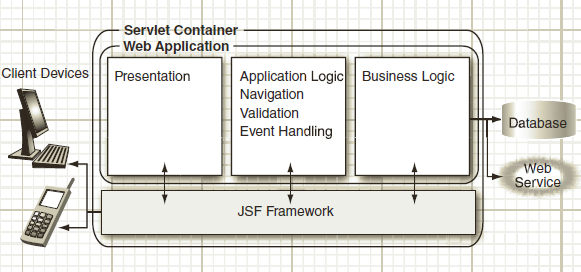
\includegraphics{JSF_architecture.png}
	\caption{Architettura di JSF}
	\label{jsf_arch}
\end{figure}

L'architettura di JSF (illustrata in Figura \ref{jsf_arch} ) segue il classico schema \textit{Model-View-Controller}: JSF consente di collegare il modello (\textit{model}) con l'interfaccia grafica (\textit{view}), fornendo gli strumenti necessari per poter controllare e processare le azioni degli utenti e aggiornare il modello sottostante di conseguenza (\textit{controller}). Tali strumenti realizzano principalmente tre tipi di servizi:

\begin{itemize}
\item \textbf{gestione degli eventi}: interagendo con la pagina web, l'utente può compiere una grande varietà di azioni; esse vengono rilevate dal browser, che \textquoteleft lancia\textquoteright{} il relativo evento. JSF consente di elaborare la risposta del programma tramite un meccanismo molto semplice: è possibile associare ad un dato evento un metodo di un oggetto Java lato server che si occupa della sua gestione.
\item \textbf{conversione dei dati}: nel web, i dati vengono immessi, visualizzati e scambiati sotto forma di stringa; il modello dei dati, invece, è composto da oggetti Java. JSF permette in modo agevole di effettuare le conversioni necessarie per consentire l'interazione tra questi due mondi: oltre a fornire dei convertitori per i tipi basilari (come ad esempio numeri o stringhe), offre anche la possibilità di definire convertitori personalizzati.
\item \textbf{validazione dei dati}: viene realizzata in modo simile alla conversione: lo sviluppatore può decidere di utilizzare i \textit{validator} standard o implementarne di nuovi. Tramite questo meccanismo si evita che gli errori dell'utente pregiudichino la validità del modello.
\end{itemize}


\subsubsection{Bean}

Il livello \textit{controller} di JSF fa un uso intensivo dei \textsl{bean}. Un bean è un oggetto Java gestito dal framework e non in maniera diretta dal programmatore.\\
Esistono vari tipi di bean; quelli a cui si può accedere direttamente da una pagina JSF sono detti \textit{managed bean}. Per essere tale, un bean deve avere un nome ed uno \textit{scope}, ossia un contesto in cui il bean è \textquoteleft visibile\textquoteright{} ed utilizzabile dall'applicazione. \\
Per maggiori dettagli, si rimanda al capitolo INSERIRE RIFERIMENTO A CDI QUI.


\subsection{Funzionamento}

\subsubsection{\textit{Rendering} delle pagine}
Ci sono diversi modi per creare una pagina JSF. Quello standard fa uso della tecnologia \textsl{Facelets}, che è stata sviluppata proprio per essere utilizzata da JSF; per creare una pagina Facelets è infatti sufficiente scrivere un documento XHTML che fa uso dei tag di JSF, con la possibilità di utilizzare l'\textsl{Expression Language} (\textsl{EL}) per consentire la comunicazione tra il livello presentazione e il livello applicazione. Ciascun tag è associato ad una classe che lo gestisce e le istanze di queste classi sono dette \textit{tag handler}: quando la pagina viene letta, i \textit{tag handler} vengono eseguiti e costruiscono un albero dei componenti della pagina (\textit{component tree}). Ad ogni tag corrisponde un nodo dell'albero. Ogni componente è inoltre associato ad un oggetto \textit{renderer}, che produce codice HTML in relazione allo stato del componente stesso (processo che viene detto \textit{encoding}).\\
La pagina così prodotta arriva all'utente. Quando l'utente invia dati al server, questo processa la richiesta e produce una serie di coppie ID/valore che viene memorizzata in una tabella hash. Ciascun componente può quindi consultarla e stabilire quali sono i valori relativi al tag ad esso associato, salvandoli come \textsl{valori locali} (o \textit{local values}). Questa operazione è chiamata \textit{decoding}.\\

\begin{figure}
	\centering
	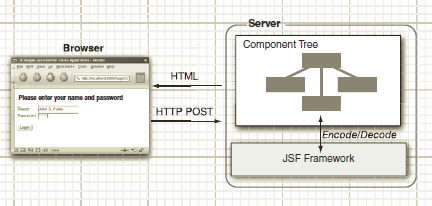
\includegraphics{JSF_client-server_communication.png}
	\caption{\textit{Encoding} e \textit{decoding}}
	\label{jsf_cs_comm}
\end{figure}

\subsubsection{\textit{Comunicazione client-server}}
La comunicazione tra client e server può avvenire essenzialmente in due modi, entrambi standard: tramite richieste \textsl{POST} e \textsl{GET}. JSF inoltre supporta nativamente ed in modo trasparente le richieste AJAX, consentendo di creare pagine web dinamiche. La comunicazione asincrona tramite AJAX è uno strumento molto efficace in vari contesti; la figura \ref{jsf_ajax} mostra come possa ad esempio essere utilizzata per la gestione degli eventi e la validazione dei dati.\\

\begin{figure}
	\centering
	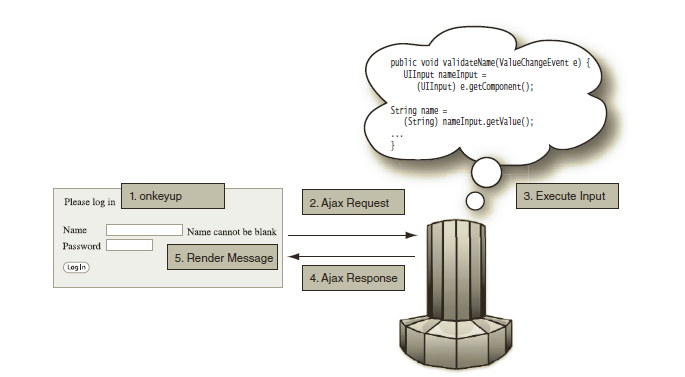
\includegraphics{JSF_ajax.png}
	\caption{Richiesta AJAX per la validazione di un input}
	\label{jsf_ajax}
\end{figure}

\subsubsection{\textit{Ciclo di vita}}
Ciò che viene eseguito tra una richiesta HTTP e la relativa risposta è chiamato dalla specifica JSF \textsl{ciclo di vita} (in inglese \textit{life cycle}).
Di seguito vengono riportate le sei fasi del ciclo di vita di JSF (raffigurate nella figura \ref{jsf_lifecycle}), come stabilito dalla specifica:

\begin{enumerate}
\item \textbf{\textit{Restore view}}: è la fase in cui viene costruito l'albero dei componenti, o viene recuperato nel caso di pagina mostrata precedentemente.
\item \textbf{\textit{Apply request values}}: in questa fase, la richiesta HTTP che l'utente invia al server viene processata, eseguendo l'operazione di \textit{decoding}.
\item \textbf{\textit{Process validations}}: viene eseguita la conversione e la validazione dei dati dell'utente.
\item \textbf{\textit{Update model values}}: durante questa fase viene aggiornato il modello dei dati.
\item \textbf{\textit{Invoke application}}: è la fase in cui il \textit{navigation handler} di JSF decide quale pagina visualizzare in base alle decisioni prese dal controllore.
\item \textbf{\textit{Render response}}: viene eseguito l'\textit{encoding}, producendo una pagina HTML che viene poi inviata al browser tramite la risposta del server.
\end{enumerate}

\begin{figure}
	\centering
	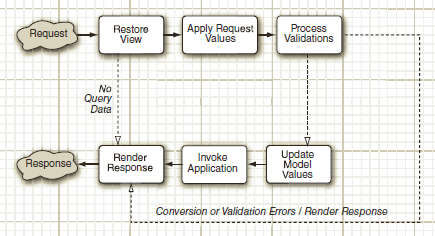
\includegraphics{JSF_life_cycle.png}
	\caption{Ciclo di vita di JSF}
	\label{jsf_lifecycle}
\end{figure}

Non sempre vengono eseguite tutte le fasi del ciclo di vita. Alcuni esempi:

\begin{itemize}
\item Nel caso in cui la richiesta HTTP non contenga valori, a seguito della fase \textit{Restore view} viene eseguita immediatamente la fase \textit{Render response}. Ciò accade, ad esempio, quando una pagina viene visualizzata per la prima volta.
\item Se si riscontrano errori di conversione o validazione durante la fase \textit{Process validations}, si passa alla fase \textit{Render response}: viene visualizzata nuovamente la stessa pagina, mostrando i relativi messaggi di errore (se previsti nella creazione della pagina stessa da parte dello sviluppatore).
\item In una richiesta AJAX vengono indicati quali componenti processare e quali aggiornare. Per i primi vengono eseguite le prime cinque fasi del ciclo di vita e successivamente viene eseguito il \textit{rendering} solo per i componenti da aggiornare.
\end{itemize}

















\section{Deltaspike}
\textsl{Deltaspike} è un \textit{framework} che estende le funzionalità di \textsl{CDI}. Il suo utilizzo in Jama è la gestione della sicurezza: associare ad ogni utente un insieme di permessi che determinano le azioni che può effettuare.
La caratteristica fondamentale di Deltaspike è l'essere un \textit{framework annotation-based}: funziona tramite le \textsl{Annotation} di Java - che d'ora in poi chiameremo semplicemente annotazioni - il che lo rende facile da utilizzare e poco invasivo.

\subsection{Caratteristiche Generali}
Il cuore della sicurezza in Deltaspike è la classe \textsl{Authorizer}: è un \textit{bean} di CDI - tipicamente \textsl{Application Scoped} - definito dallo sviluppatore che definisce i metodi che verranno invocati durante il controllo sui permessi di un utente. Questi metodi devono essere annotati con l'annotazione \textsl{@Secures} definita da Deltaspike, che indica che essi sono i metodi da invocare per il controllo sui permessi. Non basta: devono essere annotati anche con un'altra annotazione, una \textsl{custom annotation} - cioè definita dallo sviluppatore - che associa il metodo in questione ai metodi su cui effettuare il controllo dei permessi. Quest'ultima deve essere a sua volta annotata con l'annotazione \textsl{@SecurityBindingType} di Deltaspike.\newline
Nonostante già il controllo sui metodi possa essere sufficiente per gestire l'intera sicurezza di un'applicazione, una funzionalità interessante e molto utile di Deltaspike è la possibilità di effettuare un controllo a livello di pagina: ad esempio, far sì che solo un Amministratore possa visitare la pagina di creazione di un utente, o che solo un Operatore Amministrativo possa visitare la pagina di creazione di una convenzione. Inoltre, qualora il controllo non vada a buon fine, si può specificare una pagina di errore diversa per ogni pagina, ed un messaggio di errore che verrà visualizzato a video dopo il redirect.\newline
Per concludere quest'introduzione e visione d'insieme delle funzionalità di Deltaspike con cui abbiamo avuto a che fare, riteniamo comunque importante far notare che, nonostante sia un framework già usabile e utile, non sia ancora completamente maturo: la documentazione è scarsa - per non dire di peggio - e alcune funzionalità utili sono mancanti o non funzionanti - ad esempio, il redirect ad una pagina di errore anche per la sicurezza sui metodi.\newline
Vediamo adesso in dettaglio come utilizzare Deltaspike.



\subsection{Rendere sicuro un metodo}
Per spiegare come si rende sicuro un metodo, prenderemo come esempio un problema che abbiamo affrontato nello sviluppo di Jama: far sì che solo un Operatore Amministrativo possa eliminare una convenzione. L'eliminazione di una convenzione, nella nostra applicazione, consiste in sostanza nell'invocazione di un metodo di uno dei nostri \textit{bean}, quindi il problema si risolve impedendo l'invocazione di tale metodo da parte di utenti che non siano un Operatore Amministrativo.\newline
Il primo passo è il definire un'annotazione, che chiameremo \textsl{@DeleteContractsAllowed}:

\begin{lstlisting}
&&Retention&&(value = RetentionPolicy.RUNTIME)
&&@Target&&({ ElementType.TYPE, ElementType.METHOD })
&&@Documented&&
&&@SecurityBindingType&&
public @interface DeleteContractsAllowed {}
\end{lstlisting}

Procediamo dunque ad annotare il nostro metodo che elimina una convenzione con l'annotazione appena definita:

\begin{lstlisting}
...

&&@DeleteContractsAllowed&&
public void deleteContract() {
	//Elimina una convenzione.
	
	...
}
\end{lstlisting}

L'ultima cosa da fare è fornire l'Authorizer di un metodo annotato \textsl{@Secures} e \textsl{@DeleteContractsAllowed}:

\begin{lstlisting}

public class Authorizer {
	&&@Secures&&
	&&@DeleteContractsAllowed&&
	public boolean canDeleteContracts {
		//Verifica che l'utente possa eliminare una convenzione.
		//Restituisce true in caso affermativo, altrimenti false.
	
		...
	}
}
\end{lstlisting}

Il metodo che abbiamo appena definito verrà invocato da Deltaspike in maniera automatica tutte le volte che si invocherà \textsl{deleteContract()}. Nel caso \textsl{canDeleteContracts()} restituisca \textsl{true}, l'eliminazione può proseguire, altrimenti viene generata un'eccezione.

\subsection{Rendere sicura una pagina} 
La sicurezza su base pagina si implementa definendo interfacce e classi che rappresentano rispettivamente cartelle e pagine. Ad esempio, per rendere sicura la pagina \textsl{home.xhtml} che si trova dentro la cartella \textsl{pages}, definiremo un interaccia \textsl{Pages} con all'interno una classe \textsl{Home}; le classi così definite devono implementare l'interfaccia \textsl{ViewConfig} definita da Deltaspike. Il \textit{path} è relativo alla cartella \textsl{webapp} dell'applicazione, quindi la nostra classe Home contenuta nell'interaccia Pages fa riferimento alla pagina \textsl{webapp/pages/home.xhtml}. I nomi sono \textit{case insensitive}: la classe Home fa riferimento alle pagine home.xhtml e Home.xhtml; stesso discorso vale per le interfacce.\newline
Il metodo più facile per rendere sicuro un insieme di più pagine è creare un file Java e di definire all'interno di quest'ultimo tutta la gerarchia di interfacce e di classi - ricordandoci di omettere il \textit{modifier} \textsl{public} per ognuna delle interfacce/classi, altrimenti si otterrebbe un errore di compilazione.\newline
Ognuna delle classi definite deve essere annotata con l'annotazione \textsl{@Secured}, completata con l'attributo \textsl{value} che specifica una classe definita dallo sviluppatore che implementa l'interfaccia \textsl{AccessDecisionVoter} di Deltaspike; questa classe deve essere un \textit{bean} di CDI, tipicamente \textsl{Application Scoped} .
La classe specificata deve implementare il metodo \textsl{public Set\textless SecurityViolation\textgreater \space checkPermission()}, che viene invocato da Deltaspike ogni volta che si tenta di accedere alla pagina.\newline
Il metodo restituisce un Set di \textsl{SecurityViolation}, una \textsl{Anonymous Inner Class} definita da Deltaspike. Nel caso esso sia vuoto, l'accesso viene consentito, altrimenti viene impedito.\newline Come abbiamo visto nell'introduzione, una delle peculiarità più interessanti della sicurezza su base pagina è il poter specificare una pagina di errore. Per fare ciò, arricchiamo l'annotazione \textsl{@Secured} delle nostre pagine con l'attributo \textsl{errorView}, indicando una pagina definita secondo la solita convenzione spiegata ad inizio paragrafo. Nel caso venga specificata una pagina di errore, le SecurityViolation contenute nel Set restituito da checkPermission() vengono aggiunte al \textit{bundle} di messaggi della pagina, ovvero all'interno dell'area definita dal tag \textsl{\textless h:messages\textgreater} della pagina - detta in maniera meno tecnica, verrà visualizzato un messaggio a video nella pagina di errore per ogni SecurityViolation contenuta. \newline Il messaggio da visualizzare viene specificato nel metodo \textsl{public String getReason()} di ogni SecurityViolation; ricordando che quest'ultima è una Anonymous Inner Class, il metodo getReason() viene obbligatoriamente ridefinito ad ogni SecurityViolation creata, permettendo così di specificare il messaggio di errore più adatto in ogni occasione.\newpage
Per fissare meglio le idee, è opportuno mostrare un esempio. Per prima cosa, creiamo le classi relative alle pagine da rendere sicure:

\begin{lstlisting}
interface Pages {

	@Secured(value = { ViewHomeAccessDecisionVoter.class }, errorView = Login.class)
	class Home implements ViewConfig {}

	
	class Login implements ViewConfig {}

}
\end{lstlisting}

Successivamente definiamo il nostro AccessDecisionVoter; non ci addentreremo nella logica che esegue il controllo, usiamo uno pseudo-codice che renda l'idea di come deve funzionare la classe:

\begin{lstlisting}
&&@ApplicationScoped&&
public class ViewHomeAccessDecisionVoter implements AccessDecisionVoter {
	private SecurityViolation violation = new SecurityViolation() {
		public String getReason() {
			return "Non sei autorizzato";
		};
		
	public Set<SecurityViolation> checkPermission(
				AccessDecisionVoterContext accessDecisionVoterContext) {
				
		Set<SecurityViolation> violations = new HashSet<>();
				
		if( user cannot see home )
			violations.add(violation);
		return violations;
	}
}

\end{lstlisting}
Il gioco è fatto: chiunque tenti di visitare la pagina \textsl{home} senza averne i permessi - ad esempio, un utente che senza fare il login tenta di andare subito alla home - viene reindirizzato alla pagina di login, dove potrà vedere un bel messaggio che recita: \textsl{Non sei autorizzato!}\newline

\chapter{Utilizzo}




\end{document}       
